\documentclass{article}
\usepackage[utf8]{inputenc}
\usepackage{graphicx}

\begin{document}

\section{Presence and location}

\subsection{Objective and Functionality}
The presence and location is a set of two devices each with an ultrasonic sensor that determine user presence and location (left-right). Each of the sensors is responsible of sending collected data to their respective topic (sensor1/distance or sensor2/distance).

\subsection{Project Definition and Milestones}
The development of the presence and location system just involves establishing an MQTT connection with the broker to send the collected data from the ultrasonic sensors.

\subsection{Achieved milestones, execution order, priority, and dependencies}
\begin{enumerate}
    \item \textbf{Milestone 1: Establishing MQTT Communication}
       - \textit{Priority:} High. Fundamental for data transmission.
       - \textit{Dependencies:} Basic WiFi setup.
       - \textit{Execution Order:} First, as it is crucial for data reception.

    \item \textbf{Milestone 2: Send the collected that from the sensor}
       - \textit{Priority:} High. Essential for functionallity
       - \textit{Dependencies:} Successful MQTT setup.
       - \textit{Execution Order:} Second, building upon established communication.
\end{enumerate}

\subsection{Hardware setup}
The hardware setup for the location and presence comprises:
\begin{itemize}
    \item Two ESP-01 modules.
    \item Two ultrasonic sensor, one for each ESP-01 module.
\end{itemize}

\subsection{Software Implementation}
The software, written in arduino programming language, has the following key functionalities:
\begin{itemize}
    \item Connect to WiFi (and try to reconnect if needed).
    \item Establish MQTT connection.
    \item Measure and calculate distance using ultrasonic sensor pins.
    \item Send the resulting data to the corresponding topic (sensor1/distance or sensor2/distance)
\end{itemize}

\subsection{Dedication Time}
Approximately 15 hours were dedicated to developing the System Monitor, mainly spent on finding out sensor malfunctioning given that the software implementation was simple and straightforward.

\subsection{Challenges and Solutions}
\begin{itemize}
    \item \textbf{Hardware Challenges:} Malfunctioning sensors which drove us crazy.
    \item \textbf{Software Challenges:} Processing sensor data accurately, since this cheap sensors can provide really confusing data.
\end{itemize}

\subsection{Hardware and Software Integration}
\begin{figure}[ht]
    \centering
    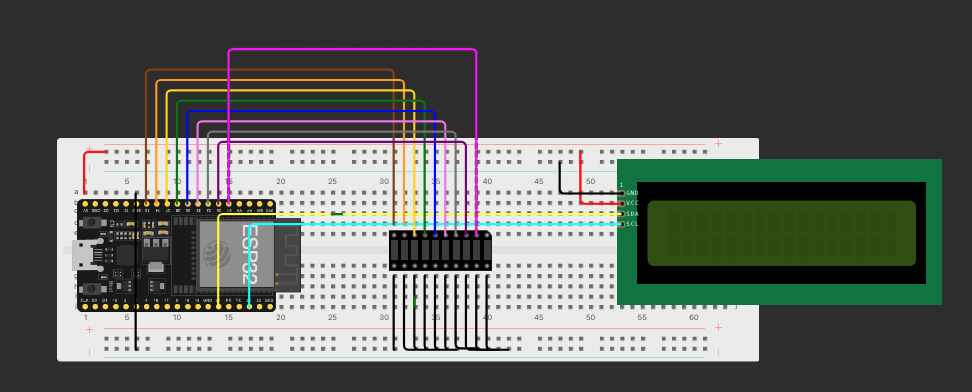
\includegraphics[width=0.8\textwidth]{../images/activity_monitor_scheme.png}
    \caption{ESP32 with LED bar and LCD display connected on a breadboard.}
    \label{fig:esp32_system_monitor}
\end{figure}

\subsubsection{Data Flow and Configuration}

\subsection{MQTT Tree Structure}
The MQTT protocol in the presence and location project uses a structured approach to manage the data flow. Below is the outline of the MQTT topics and their functions:

\subsubsection{MQTT Topics}
\begin{itemize}
    \item \textbf{sensor1/distance:} This topic is used by the first ESP-01 module. It publishes the distance data measured by its connected ultrasonic sensor.
    \item \textbf{sensor2/distance:} Similar to the first, this topic is for the second ESP-01 module.
\end{itemize}

\subsubsection{Data Organization and Utilization}
The data sent to these topics include numerical values representing the measured distances. 

\end{document}
